\section{User Guide}
This section contains descriptions of how the gravity effector code works and includes descriptions of and notes on variables. It should be helpful to users who wish to use the gravity effector module.

\subsection{Code Diagram}
The diagram in Fig. \ref{img:codeFlow} demonstrates the basic iterative logic of the gravity effector module. There is extensive additional code that deals with things from the messaging system to transforming the spacecraft position from one frame to another. In general, the inputs shown must be given for each gravity body to be considered. There are, however, convenience functions which add the standard values of these inputs for common celestial bodies. An example is simIncludeGravbody.createEarth() in the test\_scenarioOrbitManeuver.py tutorial.

After the inputs are given for each gravity body, the computeGravityInertial() method calculates the $0^{\textrm{th}}$ degree gravity term for each body and its effects on the spacecraft. If useSphericalHarmParams is True for a given body, then computeField() is called to calculate and add the non-Keplerian term higher degree spherical harmonics terms for that body. If usePolyhedral is True for a given body, then computeField() is called to compute the polyhedron gravity acceleration which overrides the previous $0^{\textrm{th}}$ degree gravity term (as it is implicitly considered in the polyhedron gravity computation). 

\begin{figure}[H]
	\centering 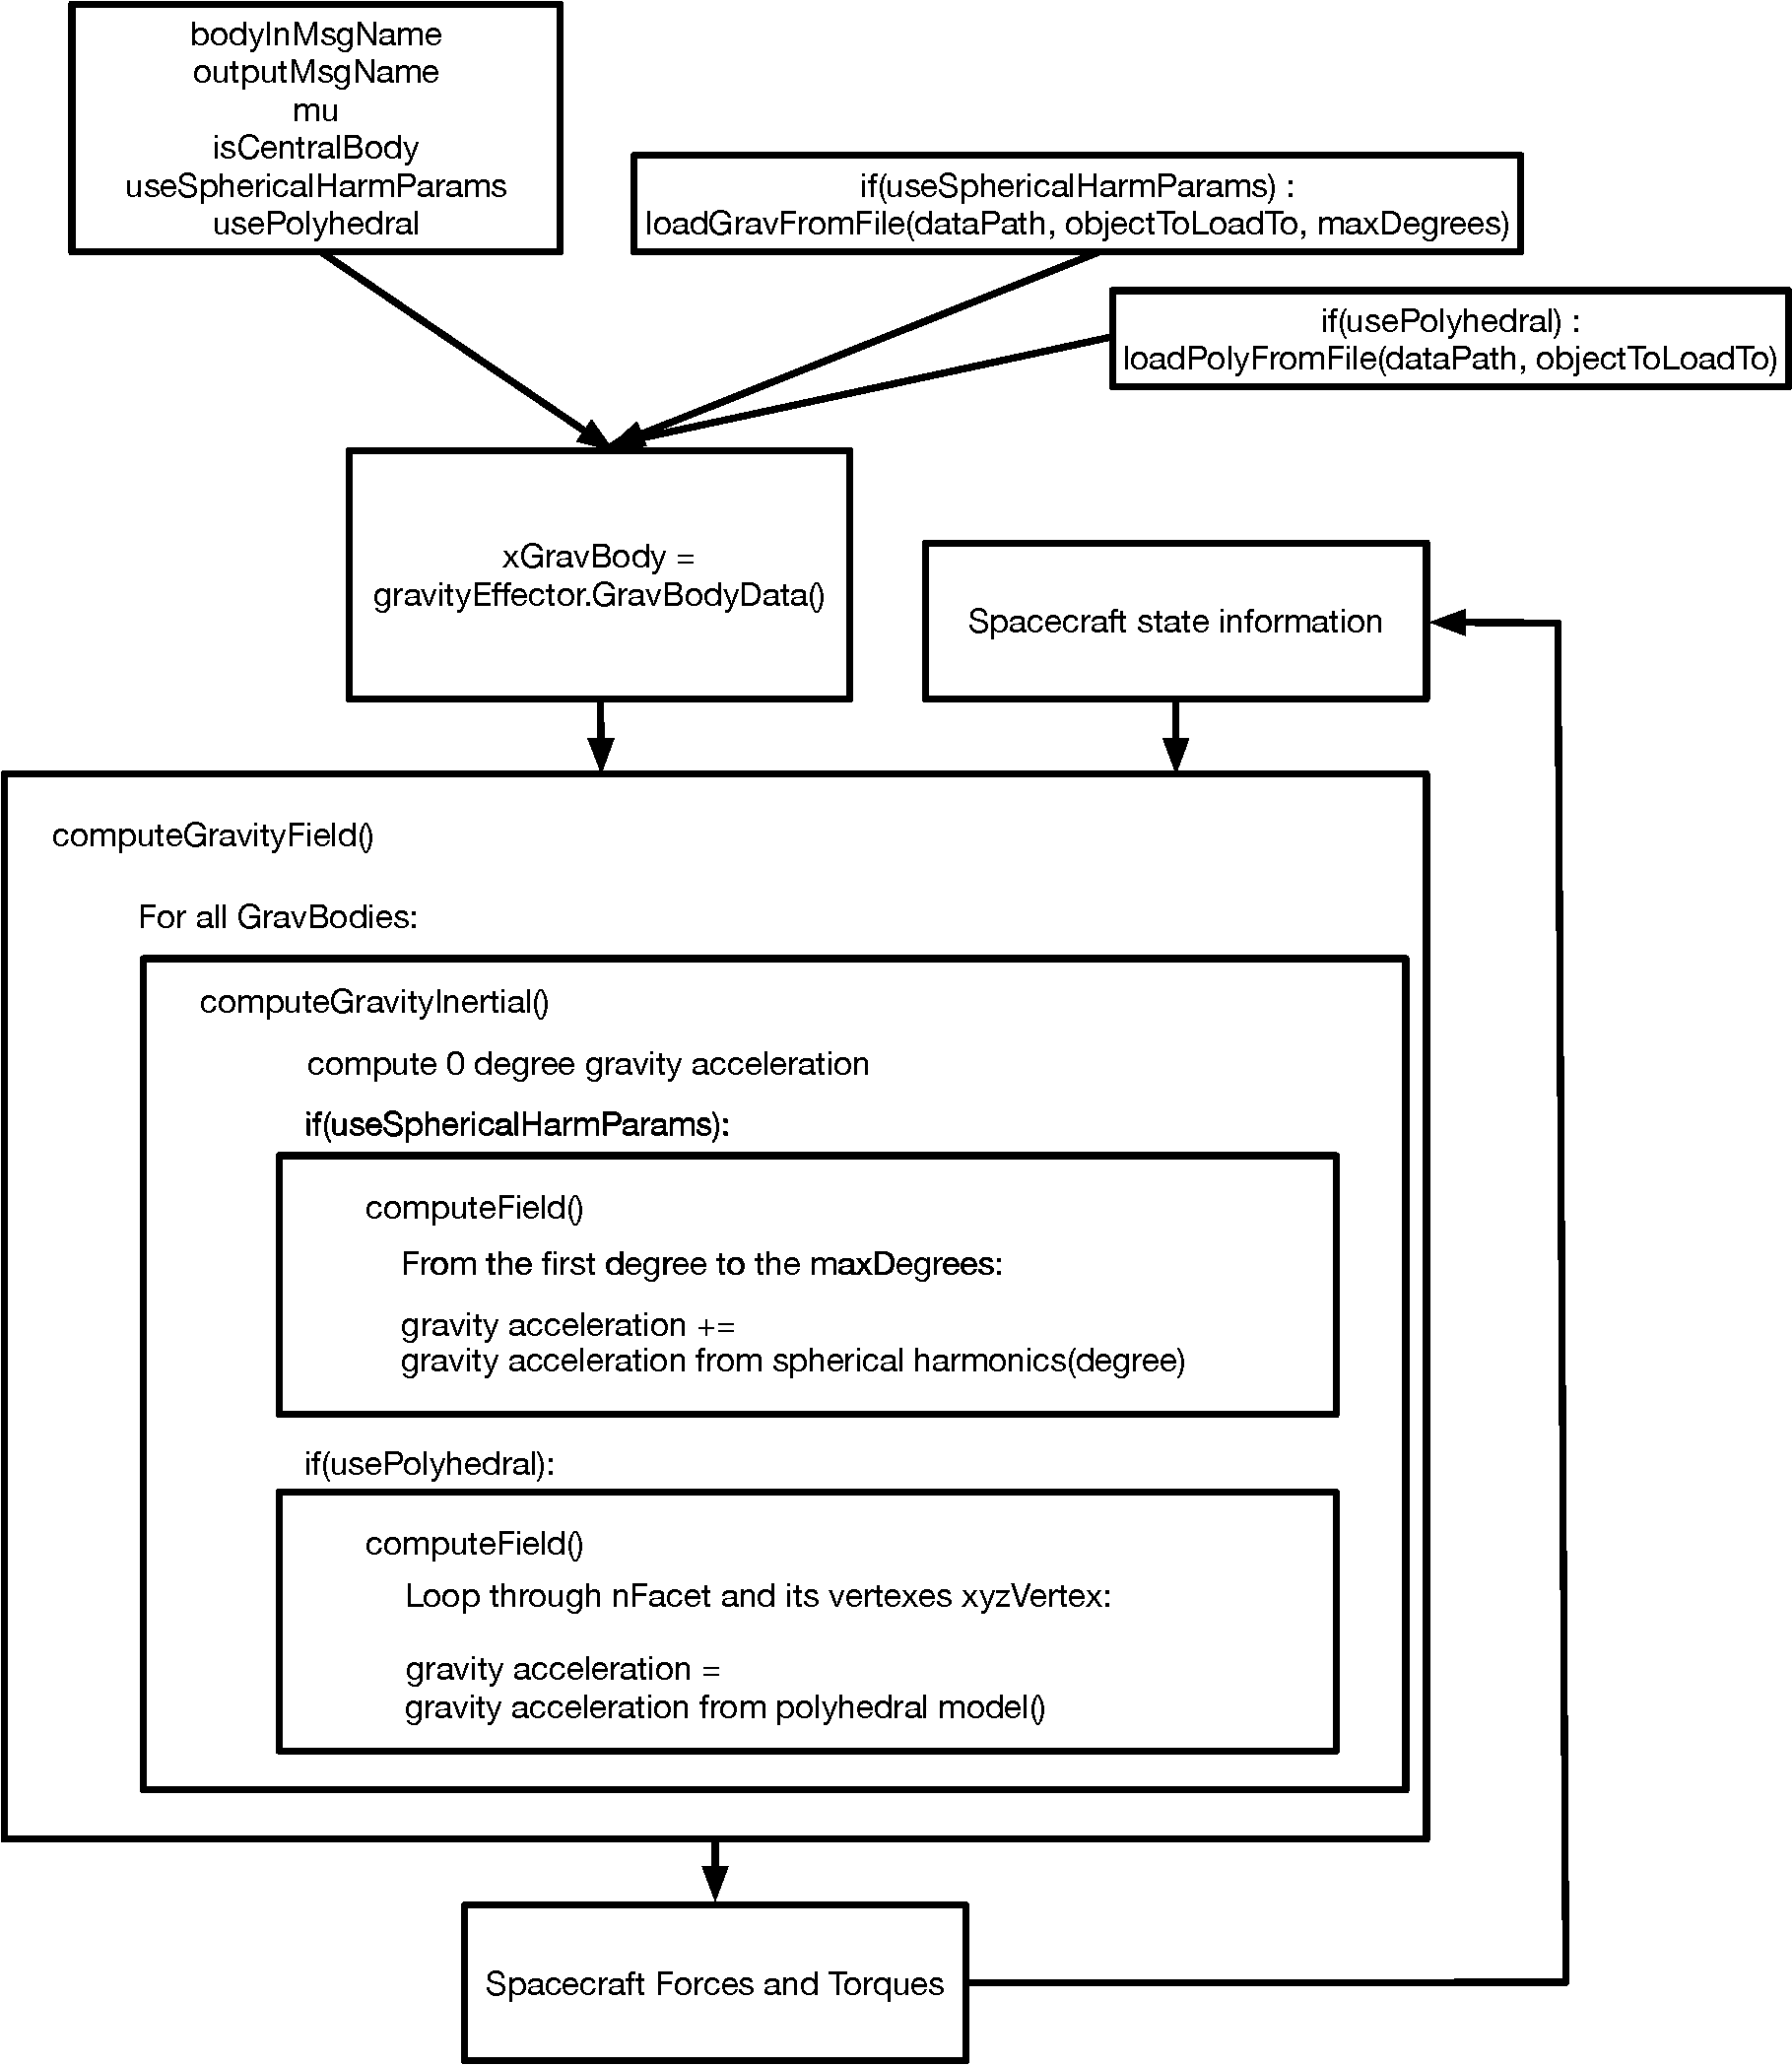
\includegraphics[height=1.0\textwidth, keepaspectratio]{Figures/codeFlow.pdf}
	\caption{A pseudo-code diagram demonstrating the flow of inputs and outputs in the gravity effector module.}
	\label{img:codeFlow}
\end{figure}

\subsection{Variable Definition and Code Description}
The variables in Table \ref{tabular:vars} are available for user input. Variables used by the module but not available to the user are not mentioned here. Variables with default settings do not necessarily need to be changed by the user, but may be.
\begin{table}[H]
	\caption{Definition and Explanation of Variables Used.}
	\label{tab:errortol}
	\centering \fontsize{10}{10}\selectfont
	\begin{tabular}{ | m{3cm}| m{3cm} | m{3cm} | m{6cm} |} % Column formatting, 
		\hline
		\textbf{Variable}   							& \textbf{LaTeX Equivalent} 	&		\textbf{Variable Type} & \textbf{Notes}			  \\ \hline
		spherHarm.maxDeg					&$l_{\text{max}}$		 	  & double & Default setting: 0"inertial\_state number of degree to use when calculating gravity effects using sperical harmonics.\\ \hline
		radEquator			   & $R_{\mathrm{ref}}^{l}$			& double & [m] Default setting: 0.0. 	This is the reference radius of the gravity body.\\ \hline
		muBody					& $\mu$ 		& double & [m3/s2] Default setting: 0.0f. This is the gravitational parameter of the body. Required Input to get any non-zero values out of the code.\\ \hline
		isCentralBody & N/A & bool & Default setting: False. Determines whether the body in question is the central body and if initial spacecraft position and velocity are determined as relative or inertial.\\ \hline
		isDisplayBody & N/A & bool & Default setting: False. Determines whether the body in question is the focus of the visualization\\ \hline
		ephemTime & N/A & double & [s] Default setting: 0. The ephemeris time for the body in question \\ \hline
		ephIntTime & N/A & double & [s] Default setting: 0. Required Input. The integration time associated with the ephem data. \\ \hline
		planetEphemName & N/A & string & Required Input. An ephemeris name for the planet (user-named). \\ \hline
		\label{tabular:vars}
	\end{tabular}
\end{table}

\subsection{Using Central Bodies and Relative Dynamics}
\subsubsection{Using Central Bodies}
In simulations with multiple planetary bodies, using dynamics relative to a central body can improve accuracy. Generally, this is the right thing to do rather than using an absolute coordinate set. If a user has a gravBody called \verb|earth|, the central body flag should be set to True.
\verb|earth.isCentralBody = True|	
The dynamics will then take care of themselves, but the user needs to be careful to input initial position and velocity values as \textit{relative to} the central body. This can be input from a set of Keplerian orbital elements using \verb|orbitalMotion.elem2rv| as in\\ \verb|Basilisk/tests/scenarios/scenarioBasicOrbit.py|. 

The user should be aware that if spacecraft position and velocity are read back from a message log or plotted that the absolute position and velocity will be returned. It will take additional work to convert the outputs back to a relative form by subtracting out the central body positions and velocities. No rotation will be needed, though.
It is critical that the relative position and velocities are given in a frame which is linearly translated but \textbf{not rotated} from the simulation inertial frame. There is no handling of rotated relative frames within the dynamics. The orbital element to position and velocity conversion in the section below can be used for relative dynamics inputs, as well.

\subsubsection{Not Using Central Bodies}
If no planets are designated as central bodies, an absolute initial position and velocity must be given. Again, \verb|orbitalMotion.elem2rv| can be used if the orbital elements are given in a frame not rotated from the simulation inertial frame. However, now, the initial position and velocity of the central body must be accounted for. These can be retrieved from spice via the planetStates utility:\\\\
\verb|oe = om.ClassicElements()|\\
\verb|oe.a = orbit_a * 1000 #m, orbit semi-major axis|\\
\verb|oe.e = orbit_e #eccentricity|\\
\verb|oe.i = radians(orbit_i) #inclination, radians.|\\
\verb|oe.Omega = radians(orbit_O) # orbit RAA, radians|\\
\verb|oe.omega = radians(orbit_o) #orbit argument of periapsis, radians|\\
\verb|oe.f = radians(orbit_f) # orbit true anomaly, radians|\\
\verb|r_sc_E, v_sc_E = om.elem2rv(muEarth, oe) #get xyz coordinates from keplerian elements|\\\\
\verb|ephemerides = spice_interface.SpiceInterface()|\\
\verb|ephemerides.ModelTag = "SpiceInterfaceData"|\\
\verb|ephemerides.SPICEDataPath = splitPath[0] + '../supportData/EphemerisData/'|\\
\verb|ephemerides.outputBufferCount = 2|\\
\verb|ephemerides.planetNames = spice_interface.StringVector(["earth", "sun"])|\\
\verb|ephemerides.UTCCalInit = simStart #pick a UTC string|\\
\verb|earthPos_N, earthVel_N = planetStates.planetPositionVelocity('EARTH', simStart)|\\
\verb|r_sc_N = array(r_sc_E).flatten() + array(earthPos_N).flatten()|\\
\verb|v_sc_N = array(v_sc_E).flatten() + array(earthVel_N).flatten()|\\
\verb|scObject.hub.r_CN_NInit = array(r_sc_N)|\\
\verb|scObject.hub.v_CN_NInit = array(v_sc_N)|\\\\
Of course, if a user has initial positions and velocities directly, those should be used. See scenarioCentralBody.py for a working example.\\

\subsubsection{Reference Frames}
An understanding of spice reference frames will help to explain the code above. The spice inertial frame is the ICRF. The ICRF is coplaner with the Earth's equator. Generally, the Earth Centered Inertial system one would give Keplerian elements in is aligned with ICRF. ICRF is referred to within spice as "j2000" for legacy reasons and because the J2000 system is only rotated from the ICRF by a few milliarcseconds.

\subsection{Loading polyhedral shape files}

The user has to load polyhedral files in a similar way as spherical harmonics ones. The following code, that loads a polyhedral shape from the file 'EROS856Vert1708Fac.txt', is shown as an example: \\\\
\verb|mu = 4.46275472004*1e5|\\
\verb|gravFactory = simIncludeGravBody.gravBodyFactory()|\\
\verb|polyBody = gravFactory.createCustomGravObject('eros', mu=mu)|\\
\verb|polyBody.usePolyhedral = True|\\
\verb|simIncludeGravBody.loadPolyFromFile('EROS856Vert1708Fac.txt', polyBody.poly)|\\

\subsubsection{Supported polyhedral shape files}

The current supported polyhedral shapes files have extensions as '.obj', '.tab' and '.txt'. These describe polyhedral shape models with triangular faces (three vertexes per face). Generally speaking, these files contain the polyhedral vertexes coordinates followed by the composition of each face (in other words, the vertexes that compose a face). It is expected that the vertexes coordinates are stated in kilometers (km). Then, the file reader function \verb|loadPolyFromFile| does the neccesary conversions to meters (m). The vertexes positions are assumed in a body-centered body-fixed reference frame, thus the $z$ coordinate is aligned with the body rotation axis. The expected format of each one of the supported files is detailed below (for a polyhedral shape of 32002 vertexes and 64000 faces).\\

The '.obj' file has to follow this format:\\
\verb|v -0.477031 0.084442 232.978500|\\
\verb|...|\\
\verb|v -1.560627 -1.586087 -225.401962|\\
\verb|f 10 9 1|\\
\verb|...|\\
\verb|f 32002 31996 32000|\\

The '.tab' file has to follow this format:\\
\verb|1 -0.477031 0.084442 232.978500|\\
\verb|...|\\
\verb|32002 -1.560627 -1.586087 -225.401962|\\
\verb|1 10 9 1|\\
\verb|...|\\
\verb|64000 32002 31996 32000|\\

The '.txt' file has to follow this format:\\
\verb|32002 64000|\\
\verb|-0.477031 0.084442 232.978500|\\
\verb|...|\\
\verb|-1.560627 -1.586087 -225.401962|\\
\verb|10 9 1|\\
\verb|...|\\
\verb|32002 31996 32000|\\
